\documentclass[11pt]{article}
\usepackage[margin=1in]{geometry}
\usepackage{amsmath,amssymb,amsthm}
\usepackage{graphicx,booktabs}
\usepackage{newtxtext}
\usepackage[subscriptcorrection]{newtxmath}
\usepackage[round,authoryear]{natbib}
\usepackage{xr}
\externaldocument[M-]{main}

\newtheorem{theorem}{Theorem}
\newtheorem{proposition}{Proposition}
\newtheorem{lemma}{Lemma}
\newtheorem{corollary}{Corollary}
\renewcommand{\thetheorem}{S\arabic{theorem}}
\renewcommand{\theproposition}{S\arabic{proposition}}
\renewcommand{\thelemma}{S\arabic{lemma}}
\renewcommand{\thecorollary}{S\arabic{corollary}}
\renewcommand{\thesection}{S\arabic{section}}
\renewcommand{\thefigure}{S\arabic{figure}}
\renewcommand{\thetable}{S\arabic{table}}
\renewcommand{\theequation}{S\arabic{equation}}
\renewcommand{\proofname}{Proof}

\newcommand{\pr}{\mathrm{pr}}
\newcommand{\LC}{\mathcal{L}}
\newcommand{\var}{\mathrm{var}}

\title{Supplementary material for `Noisy calibration, latent coverage and the location of the mean'}
\author{Kun Woo Park}
\date{}

\begin{document}
\maketitle

\noindent Equation, theorem and section numbers without the prefix S refer to the main paper. Numbers that are not proved are labelled as numerical, and the precision of each computation is stated.

\section{Proofs omitted from the main paper}\label{sec:s-proofs}

\begin{proof}[Proof of Proposition~\ref{M-prop:reduction}]
Since $\mathcal F \subset \LC$ it suffices to bound the supremum over $\LC$. Let $W \in \LC$ satisfy $E\{g_x(W)\} \ge p$ and let $s < Q_q(|W|)$, so that $\pr(|W| < s) \le q - \gamma$ for some $\gamma > 0$. Choose $M \ge s$ with $g_x(w) \le p$ for $|w| \ge M$, and let $W_M$ be $W$ conditioned on $|W| \le M$, which is log-concave. With $\varepsilon_M = \pr(|W| > M)$, the conditioning removes only mass on which the kernel is at most $p$, so
\[
E\{g_x(W_M)\} \ge \frac{p - p\varepsilon_M}{1 - \varepsilon_M} = p, \qquad \pr(|W_M| < s) \le \frac{q - \gamma}{1-\varepsilon_M} < q
\]
for $M$ large. On $K = [-M, M]$ the constraint function $g_x - p$ is continuous, and $\mu \mapsto -\mu(-s, s)$ is linear and upper semicontinuous for weak convergence because $(-s,s)$ is open. By the localization theorem \citep{kannan1995, fradelizi2004}, the supremum of this functional over the log-concave probability measures on $K$ that satisfy $\int(g_x - p)\,d\mu \ge 0$ is attained at a point mass or at a law with log-affine density on a segment. Hence some member of $\mathcal F$ is feasible and has $\pr(|W| < s) < q$, that is, $Q_q(|W|) \ge s$. Since $s < Q_q(|W|)$ was arbitrary the claim follows. Only continuity of the kernel and its decay at infinity were used, so the argument applies to the average kernel $\bar g$ of \S~\ref{M-sec:hetero}.
\end{proof}

For $\beta > 0$ and $\sigma = x^{1/2}$, integration by parts gives
\begin{equation}\label{eq:closed}
\int_a^b e^{\beta w}\Phi\Big(\frac{c-w}{\sigma}\Big)dw = \frac{1}{\beta}\Big[e^{\beta w}\Phi\Big(\frac{c-w}{\sigma}\Big)\Big]_a^b + \frac{e^{\beta c + \beta^2\sigma^2/2}}{\beta}\Big\{\Phi\Big(\frac{b-c-\beta\sigma^2}{\sigma}\Big) - \Phi\Big(\frac{a-c-\beta\sigma^2}{\sigma}\Big)\Big\},
\end{equation}
so the constraint is a combination of normal distribution functions. For fixed slope and length, the translations $c$ of a member of $\mathcal F$ that satisfy the constraint form an interval, because $c \mapsto \pr(|W + c + e| \le 1)$ is log-concave \citep{prekopa1973}, and $c \mapsto \pr(|W + c| \le s)$ is log-concave, so $c \mapsto Q_q(|W + c|)$ is quasi-convex and is maximized at an end of that interval. Each end is found by a root-finding in $c$, and the quantile by a second root-finding, using \eqref{eq:closed}. This two-dimensional computation over slope and length, and an independent differential-evolution search over the three-parameter family, agree to $1.5\times10^{-13}$ at all $73$ tabulated values of $x \ge 0.006$ (numerical).

\begin{proof}[Proof of Lemma~\ref{M-lem:onesided}]
Exponential tails are log-concave, which gives one inequality. Conversely, let $Y \in \LC$ with $\pr(Y + Z \le 0) \ge p$. If $Y = y_0$ is a point mass then $y_0 \le -\Phi^{-1}(p) = \lim_{u\to\infty}\{b_u(p) - u^{-1}\log(1/q)\}$. Otherwise $F = F_Y$ is continuous and $\log F$ is concave \citep{prekopa1973}. Let $v = F^{-1}(q)$ and $G(y) = F(v + y)$. The point $0$ is interior to $\{G > 0\}$, so the right derivative $u \ge 0$ of $\log G$ at $0$ is a supergradient, and $G(y) \le q e^{uy}$ for all $y$. If $u = 0$ then $G \le q < 1$, which is impossible, so $u > 0$ and $G(y) \le \min(qe^{uy}, 1)$, which is the distribution function of $b_0 - E_u$ with $b_0 = u^{-1}\log(1/q)$. Hence $Y' = v + b_0 - E_u$ lies stochastically below $Y$ and has $q$-quantile $v$, and
\[
p \le \pr(Y + Z \le 0) \le \pr(Y' + Z \le 0) = m_u(v + b_0).
\]
Since $m_u$ is decreasing, $v \le b_u(p) - b_0$. For monotonicity, let $q' > q$, let $Y$ be feasible at $(q', q')$ with $v = F_Y^{-1}(q')$, and put $\rho = (q' - q)/(1-q)$. Then $Y$ conditioned on $Y \ge F_Y^{-1}(\rho)$ is log-concave, satisfies the constraint at level $(q' - \rho)/(1-\rho) = q$, because the removed mass has noisy constraint value at most one, and has $q$-quantile $v$. Point masses have value $-\Phi^{-1}(q') < -\Phi^{-1}(q) \le c_q$. Finally, $c_q > 0$ because $v_q(u) = u^{-1}\log\{e^{u^2/2}\Phi(b_u - u) + e^{u b_u}\Phi(-b_u)\} = u/2 + o(u)$ as $u \to 0$, where $b_u = b_u(q)$ and $u b_u \to \log(1/q)$.
\end{proof}

\begin{proof}[Proof of Theorem~\ref{M-thm:small}, lower bound]
Fix $\epsilon > 0$ and choose $u$ with $v_q(u) > c_q - \epsilon$. For $p' \in [q, (1+q)/2]$, $b_u(p') \ge b_{\min} > -\infty$. Let $Y = b_u(p') - E_u$ and $W = 1 + x^{1/2}Y$. With $\tau = 2x^{-1/2}$,
\[
\pr(|W+x^{1/2}Z| \le 1) = p' - \pr(Y + Z < -\tau) \ge p' - \eta_x, \qquad \eta_x = e^{-u(\tau + b_{\min})/2} + \Phi\{-(\tau + b_{\min})/2\},
\]
by splitting the event $Y + Z < -\tau$ according to whether $Z < -(\tau + b_{\min})/2$. Take $p' = q + \eta_x$, which lies in $[q, (1+q)/2]$ for small $x$. Since $\pr(|W| \le s) \le F_W(s)$, $Q_q(|W|) \ge 1 + x^{1/2}\{b_u(q + \eta_x) - u^{-1}\log(1/q)\}$. As $\eta_x \to 0$ and $b_u$ is continuous, $\liminf_{x\to0}\{R_{q,q}(x) - 1\}/x^{1/2} \ge c_q - \epsilon$.
\end{proof}

\begin{proof}[Proof of Lemma~\ref{M-lem:meanonesided}]
For $q > 1/2$, $v_q$ is continuous on $(0,\infty)$, tends to $0$ as $u \to 0$ and to $-\Phi^{-1}(q) < 0$ as $u \to \infty$, and is positive somewhere, so its maximizers form a nonempty compact subset of $(0,\infty)$ and $\kappa^*_q$ is well defined. Let $a = \log(1/q)$ and $A = 1 - a > 0$. Let $Y$ be nondegenerate with $q$-quantile $v$. Since $\log F_Y$ is concave, a supergradient $u > 0$ at $v$ gives $F_Y(y) \le \min\{qe^{u(y - v)}, 1\}$, the distribution function of $Y' = v + a/u - E_u$; so $Y'$ lies stochastically below $Y$ and has the same $q$-quantile. Then $E(Y') \le E(Y) \le -\kappa$ and $\pr(Y' + Z \le 0) \ge q$, so the replacement keeps both constraints. For the tail $b - E_u$ the constraints read $b \le b_u(q)$ and $b \le u^{-1} - \kappa$, so the largest quantile is $\min\{v_q(u), A/u - \kappa\}$. If $k_q(u) < \kappa$ this minimum is $A/u - \kappa$; since $k_q$ is continuous and $k_q(s) \to \infty$ as $s \to 0$, some $s < u$ has $k_q(s) = \kappa$, where the value is $A/s - \kappa > A/u - \kappa$. So only $u$ with $k_q(u) \ge \kappa$ matter, and there the value is $v_q(u)$. A point mass $y_0$ satisfying the constraints has $y_0 = E(Y) \le -\kappa \le 0 < L_q(\kappa)$, where positivity holds because $v_q(u) \sim u/2$ and $k_q(u) \sim A/u$ as $u \to 0$. Since $m_u(b) \ge \Phi(-b)$, $b_u(q) \ge -\Phi^{-1}(q)$, so $k_q$ is bounded on $[u_0, \infty)$ for every $u_0 > 0$ and $k_q(u) \ge \kappa$ forces $u \to 0$ as $\kappa \to \infty$; moreover $u b_u(q) \to \log(1/q)$, so $k_q(u) = \{A + o(1)\}/u$, and $v_q(u) = u/2 + o(u)$ as $u \to 0$ (proof of Lemma~\ref{M-lem:onesided}). These expansions give $\kappa L_q(\kappa) \to A/2$: for large $\kappa$ only small $u$ are feasible, $u \le \{A + o(1)\}/\kappa$, and $v_q(u) \le \{1 + o(1)\}u/2$ with equality at the boundary. Monotonicity is clear, and $L_q(\kappa) = c_q$ while a maximizer of $v_q$ is feasible.
\end{proof}

\begin{proof}[Proof of Proposition~\ref{M-prop:centred}]
Near $\pm r_0$ the density $f$ of $W$ is smooth with $f' = \beta f$, and the ends of the support are at positive distance. The jumps of the density at the ends of the support contribute $O\{v^{1/2}\phi(d_0/v^{1/2})\}$ near $\pm r_0$, where $d_0 > 0$ is the distance from $\pm r_0$ to the ends, which is $o(v)$. Hence $H_v(r) = \pr(|W + v^{1/2}Z| \le r) = H_0(r) + v\{f'(r) - f'(-r)\}/2 + o(v)$ uniformly near $r_0$, and the noisy quantile is $t(v) = r_0 - v\,\beta\{f(r_0) - f(-r_0)\}/[2\{f(r_0) + f(-r_0)\}] + o(v) = r_0 - (\beta v/2)\tanh(\beta r_0) + o(v)$. Scaling by $t(v)$ and writing $x = v/t(v)^2$, a continuous and increasing function of $v$ near $0$, gives the expansion. As $\beta\ell \to 0$, $W/\ell$ tends to the uniform law on $[-1/2, 1/2]$, whose $q$-quantile of $|W|/\ell$ is $q/2 < 1/2$.
\end{proof}

\begin{proof}[Proof of Theorem~\ref{M-thm:transition}, the limit]
For the lower bound in the limit, take $u$ with $k_q(u) \ge \kappa$ and the law $W = 1 + x^{1/2}\{b_u(q + \eta_x) - E_u\}$ of the lower bound in Theorem~\ref{M-thm:small}. Its mean is $1 + x^{1/2}\{b_u(q + \eta_x) - u^{-1}\} \le 1 - \kappa x^{1/2}$, because $b_u$ decreases in its argument, and it is positive for small $x$; hence $\liminf_{x\to0} x^{-1/2}\{R^{(b_x)}_{q,q}(x) - 1\} \ge v_q(u)$ for every such $u$.

For the upper bound, suppose that $x_n \to 0$, $h_n = x_n^{1/2}$, and that $W_n$ is feasible for $R^{(b_{x_n})}_{q,q}(x_n)$ with $Q_q(|W_n|) - 1 \ge a_0 h_n$, where $L_q(\kappa) < a_0 < 1$. By \eqref{M-eq:necessary}, $\kappa h_n \le 1 - |E(W_n)| \le K h_n$ with $K = (1 - a_0^2)/(2a_0)$. Replacing $W_n$ by $-W_n$ if necessary, $E(W_n) \ge 0$; let $Y_n = (W_n - 1)/h_n$, so that $-K \le E(Y_n) \le -\kappa$. The law of $T_n = Y_n + Z$ is in $\mathcal B$, with a smooth positive density of maximum $M_n$ and distribution function $F_n$, and $F_n(0) \ge \pr(|W_n + h_nZ| \le 1) \ge q$ while $F_n\{E(T_n)\} \le 1 - e^{-1}$ by the first part. So $q - 1 + e^{-1} \le F_n(0) - F_n\{E(T_n)\} \le M_n K$. For a law in $\mathcal B$ with smooth density $g$, maximum $M$ and median $m$, the hazard $g/(1 - F)$ is nondecreasing, so $g(y) \le 2g(m)\{1 - F(y)\} \le 2g(m)$ for $y \le m$, and $g/F$ is nonincreasing, which gives the same for $y \ge m$; so $g(m) \ge M/2$; the tangent bounds for $\log F$ and $\log(1-F)$ at $m$ give $\pr(|T - m| > y) \le e^{-2g(m)y}$, hence $\var(T) \le 1/\{2g(m)^2\} \le 2/M^2$. Thus $\var(Y_n) \le 2K^2/(q - 1 + e^{-1})^2$, the $Y_n$ are tight and uniformly integrable, and along a subsequence $Y_n \to Y$ in distribution with $Y \in \mathcal B$, possibly a point mass, since $\mathcal B$ is closed under weak convergence \citep{saumard2019}, $E(Y) \le -\kappa$ and $\pr(Y + Z \le 0) = E\{\Phi(-Y)\} \ge q$. On $\{W_n \ge 0\}$, whose probability tends to one, $(|W_n| - 1)/h_n = Y_n$, so $a_0 \le \{Q_q(|W_n|) - 1\}/h_n \to Q_q(Y) \le L_q(\kappa)$ by Lemma~\ref{M-lem:meanonesided}, where the quantile converges because a law in $\mathcal B$ has a unique $q$-quantile or is a point mass. This contradicts $a_0 > L_q(\kappa)$, so $\limsup_{x\to0} x^{-1/2}\{R^{(b_x)}_{q,q}(x) - 1\} \le a_0$ for every $a_0 \in (L_q(\kappa), 1)$; if $L_q(\kappa) \ge 1$ there is nothing to prove, because \eqref{M-eq:necessary} gives $\delta < x^{1/2}$.
\end{proof}

\subsection*{Ranks for Proposition~\ref{M-prop:unknown}}

At $q = 0.9$ and $\delta = 0.05$ no rank satisfies $p_k \ge 0.901$ and $k \ge Kp_k + 1$ for $K \le 28$, since even $k = K$ gives $p_K = 0.05^{1/K} < 0.901$. For every $K$ from $29$, where the rank is $k = K$, to $3000$ a rank exists, and it is at most three ranks above the usual rank with $p_k \ge 0.9$; for instance $46$ against $45$ at $K = 46$ and $2731$ against $2728$ at $K = 3000$. The gap grows with $K$, to $10$ at $K = 10^4$ ($9060$ against $9050$), because the slack $10^{-3}$ becomes large relative to the spacing of the levels $p_k$. The function \texttt{certified\_rank} returns this rank.

\begin{proof}[Proof of Proposition~\ref{M-prop:beta}]
$\bar F(T) < p_k$ exactly when $N = \#\{i : |V_i| < \bar F^{-1}(p_k)\} \ge k$. $N$ is a sum of independent indicators whose success probabilities average $p_k$, and $k - 1 \ge Kp_k$. By \citet{hoeffding1956}, $\pr(N \le k-1)$ is smallest when all success probabilities are equal. Hence $\pr(N \ge k) \le \pr\{{\rm Bin}(K, p_k) \ge k\} = \pr\{{\rm Beta}(k, K+1-k) \le p_k\} = \delta$.
\end{proof}

\subsection*{The case $p > q$}

The constant of \S~\ref{M-sec:slack} is
\[
C_{p,q} = \sup_{\alpha_L+\alpha_R = 1-p}\ \inf_{\beta_L+\beta_R=1-q} \max(c_{1-\alpha_L,1-\beta_L},\, c_{1-\alpha_R,1-\beta_R}).
\]
Numerically the worst split puts the whole budget on one end, so that $C_{p,q} = c_{p,q}$; this observation is not used. Ball arithmetic gives $-0.0572 \le C_{0.9036,0.9} \le -0.057$, where $0.9036$ is the order-statistic level for $K = 110$, $k = 105$ at $\delta = 0.04$, used in \S~\ref{sec:s-hetero}.

In the proof of the upper bound of Theorem~\ref{M-thm:small}, replace $1 - q$ by $1 - p$ for the noisy budget, choose any split $\beta_L + \beta_R = 1 - q$ of the latent budget, and use $F_Y^{-1}(1-\beta_R) \le c_{1-\alpha_R, 1-\beta_R}$ at each end. Since $c_{p',q'}$ decreases in $p'$, the worst case has $\alpha_L + \alpha_R = 1 - p$, which gives $R_{p,q}(x) \le 1 + C_{p,q}x^{1/2}$ for every $x$, with $C_{p,q}$ nonincreasing in $p$. The proof of the lower bound applies with $b_u(q)$ replaced by $b_u(p)$ and $p' = p + \eta_x$, giving $R_{p,q}(x) \ge 1 + c_{p,q}x^{1/2} - o(x^{1/2})$ for every $p \ge q$. This proves Corollary~\ref{M-cor:slack}, whose numerical intervals are certified in \S~\ref{sec:s-ball}.

\subsection*{Bi-log-concave laws}

\begin{corollary}\label{cor:blc}
Let $\mathcal B$ be the class of laws that are point masses or have a continuous distribution function $F$ with $\log F$ and $\log(1-F)$ concave \citep{dumbgen2017}; $\LC \subset \mathcal B$. Define $R^{\mathcal B}_{p,q}$ by \eqref{M-eq:R} with $\mathcal B$ in place of $\LC$. Then Lemma~\ref{M-lem:onesided} holds over $\mathcal B$ with the same $c_{p,q}$, and for $p \ge q$ and every $x > 0$, $R^{\mathcal B}_{p,q}(x) \le 1 + C_{p,q}x^{1/2}$, while $R^{\mathcal B}_{q,q}(x) = 1 + c_qx^{1/2} + o(x^{1/2})$ as $x \to 0$. In particular Corollary~\ref{M-cor:slack} holds over $\mathcal B$.
\end{corollary}

\begin{proof}
The proof of Lemma~\ref{M-lem:onesided} uses only the concavity of $\log F_Y$ at the $q$-quantile, so its upper bound holds for every $Y$ with $\log F_Y$ concave, and exponential tails are in $\LC$, which gives equality. In the proof of Theorem~\ref{M-thm:small}, $Y = (W - 1)/x^{1/2}$ has $\log F_Y$ concave, and $(-W - 1)/x^{1/2}$ has a concave log distribution function because $\log(1 - F_W)$ is concave and $F_W$ is continuous. The lower bound uses laws in $\LC \subset \mathcal B$.
\end{proof}

The class $\mathcal B$ contains multimodal laws. Proposition~\ref{M-prop:reduction} and the box-bound upper bounds of \S~\ref{sec:s-cert} use log-concavity of the density; the ball-arithmetic constants do not (Corollary~\ref{cor:blc}). Theorems~\ref{M-thm:mean} and~\ref{M-thm:transition}, Lemma~\ref{M-lem:meanonesided}, Proposition~\ref{M-prop:unknown} and Corollary~\ref{M-cor:simple} hold over $\mathcal B$: their proofs use the monotone hazards of $\mathcal B$, the bound $f' \le f^2/F$ of \citet{dumbgen2017}, and the preservation of $\mathcal B$ under convolution with a log-concave law and under weak limits \citep{saumard2019}.

Symmetry alone does not make noisy calibration conservative in $\mathcal B$. The density $f(w) = \{1 + 0.05\cos(2\pi w)\}/2$ on $(-1, 1)$ is in $\mathcal B$, because $\sup|f'| = 0.05\pi < \inf f^2 = 0.2256$ \citep[][Theorem~1]{dumbgen2017}, but it is not unimodal. At $q = 0.7$, $r_0 = Q_q(|W|) \approx 0.7077$ and $f'(r_0) > 0$; since $f'$ is odd, $\partial_s \pr(|W + s^{1/2}Z| \le r_0) = f'(r_0) > 0$ at $s = 0$, so noise raises the coverage and the noisy quantile falls below $r_0$, to $0.707676$ at $s = 10^{-5}$, against $r_0 = 0.707678$. Anderson's comparison needs unimodality. The bimodal law of Table~\ref{M-tab:synth}, the mixture $0.4\,N(m_1, s^2) + 0.6\,N(m_2, s^2)$ with mean zero, variance one and $(m_2 - m_1)/s = 2.5$, is in $\mathcal B$ by the same criterion, $f'F \le f^2$ and $-f'(1-F) \le f^2$, checked on a grid of spacing $4\times10^{-5}$ on $[-8, 8]$ (test suite); with $p = 0.4$ the mixture stays in $\mathcal B$ up to a separation of about $2.59$, where $\max(f'F - f^2)/f^2$ changes sign, while bimodality starts at about $2.443$; at $2.5$ the largest value of $(f'F - f^2)/f^2$ and of $\{-f'(1-F) - f^2\}/f^2$ is $-0.036$. The parameters are $m_1 = -0.94868$, $m_2 = 0.63246$ and $s = 0.63246$. The bound of Theorem~\ref{M-thm:mean} with $E(W) = 0$ holds for this law and its version with the cosine phase-shifted by $\pi/2$ and recentred to mean zero, at $q = 0.3, 0.7, 0.9$ and $s = 10^{-3}, 0.1, 1$ (test suite).

\section{The shape of the sharp radius}\label{sec:s-shape}

Figure~\ref{fig:s-boundary} shows $R_{q,q}(x) - 1$ computed by grid maximization over the extremal family; grid values bound $R_{q,q}$ from below. The levels at which the grid value crosses $1$ are $x^*(q) \approx 0.034$, $0.017$, $0.0062$ and $0.0012$ for $q = 0.8$, $0.85$, $0.9$ and $0.95$, and the largest widening found is $0.37\%$, $0.17\%$, $0.063\%$ and $0.012\%$. At $q = 0.9$ the numerical upper bounds of \S~\ref{sec:s-cert} give $R_{q,q}(x) \le 1$ for $x \ge 0.013$, so Theorem~\ref{M-thm:small} bounds the widening by $c_{0.9}\,0.013^{1/2} < 0.22\%$ at every $x$; this rests on the double-precision bounds, whereas the bound $1.16\%$ of \S~\ref{M-sec:mean} rests only on Theorem~\ref{M-thm:small} and the certified $c_{0.9}$. Below $x^*(q)$ the noisy threshold must be widened; above it, grid values below $1$ do not by themselves show that shrinking is safe, which the numerical upper bounds of \S~\ref{sec:s-cert} do. The exact grid values lie below $1 + c_{0.9}x^{1/2}$ at $x = 10^{-6}, \ldots, 10^{-2}$, as Theorem~\ref{M-thm:small} requires.

\begin{figure}[t]
\centering
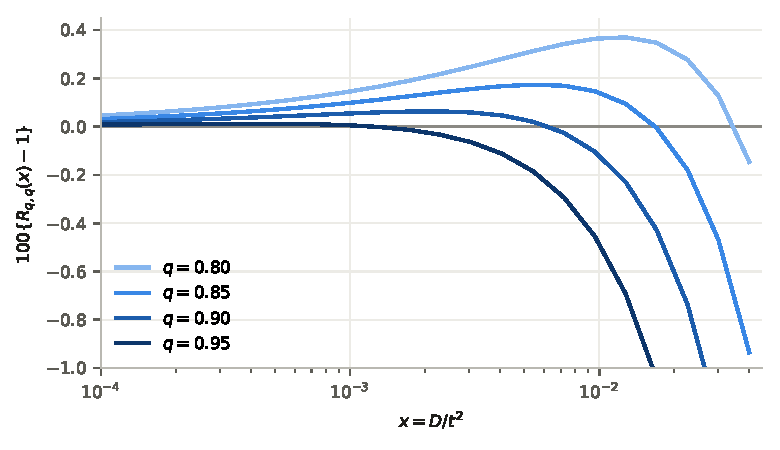
\includegraphics[width=0.7\textwidth]{fig_boundary.pdf}
\caption{Sharp latent radius relative to the noisy threshold, $100\{R_{q,q}(x) - 1\}$, for four coverage levels, computed by grid maximization over the extremal family, which bounds $R_{q,q}$ from below.}
\label{fig:s-boundary}
\end{figure}

\subsection*{Centred laws and the transition}

The following values are computed in double precision by \texttt{experiments/e32\_centering.py} and are not certified. For $q = 0.8$, $0.9$ and $0.95$: $\kappa^*_q = 6.8118$, $20.1823$ and $50.0741$, attained at $u^* = 0.11328$, $0.044286$ and $0.018943$. The two upper bounds in Fig.~\ref{M-fig:transition} cross at $\kappa = 10.829$, $26.221$ and $59.466$, where $L_q/U_q$ is smallest, $0.770$, $0.879$ and $0.927$; as $\kappa \to \infty$ the ratio tends to $1 - \log(1/q) = 0.777$, $0.895$ and $0.949$. At $q = 0.9$, $L_q(25) = 0.017393$ and $L_q(50) = 0.0089448$. For the mean-zero laws of Proposition~\ref{M-prop:centred}, the coefficient with $\beta = 0.2$ and $\ell = 2$ at $q = 0.9$ is $0.0156540$; the expansion is accurate to $6\times10^{-5}$ at $x = 1.3\times10^{-4}$ but fails at $x \approx 1.1\times10^{-3}$, where the noise reaches the end of the support and the threshold may already be shrunk. The bound of Theorem~\ref{M-thm:mean}, including its form with $|E(W)| \le B$, was checked on $642$ laws from the family of Proposition~\ref{M-prop:centred}, with no violation.

\subsection*{The location of the mean in examples}

Figure~\ref{fig:s-mean} shows the radius correction for laws scaled so that the noisy coverage of $[-1, 1]$ is exactly $0.9$, computed from closed forms by \texttt{experiments/e35\_mean\_location.py}. For the boundary-layer law $W = 1 + x^{1/2}\{b - E_u\}$ at the maximizer $u^*$ of $v_q$, whose mean lies $20.18\,x^{1/2}$ from the boundary, the correction divided by $x^{1/2}$ is $0.019062$ for $x \le 3\times10^{-5}$, equal to $c_{0.9}$. For the same family at the rate with $k_q(u) = 50$ it is $0.008945 = L_{0.9}(50)$. For the fixed mean-zero law of Proposition~\ref{M-prop:centred} with $\beta\ell = 0.5$ on a unit segment, the correction divided by $x$ is $0.024005$ up to $x = 5\times10^{-5}$, and it turns negative once the noise reaches the end of the support. Larger centred coefficients sit closer to that end: at $\beta\ell = 0.9$ the coefficient is $0.070$ but the quantile lies $0.0011$ from the end, and the correction is positive only for $x$ below about $10^{-7}$. A Gaussian law with mean $1.29\,x^{1/2}$ from the boundary after scaling, $W \sim N(1 - 2x^{1/2}, 0.01x)$ before scaling, needs no correction at all: its radius is $1.16\,x^{1/2}$ below the noisy threshold. A mean near the boundary is necessary for a correction of order $x^{1/2}$, not sufficient.

\begin{figure}[t]
\centering
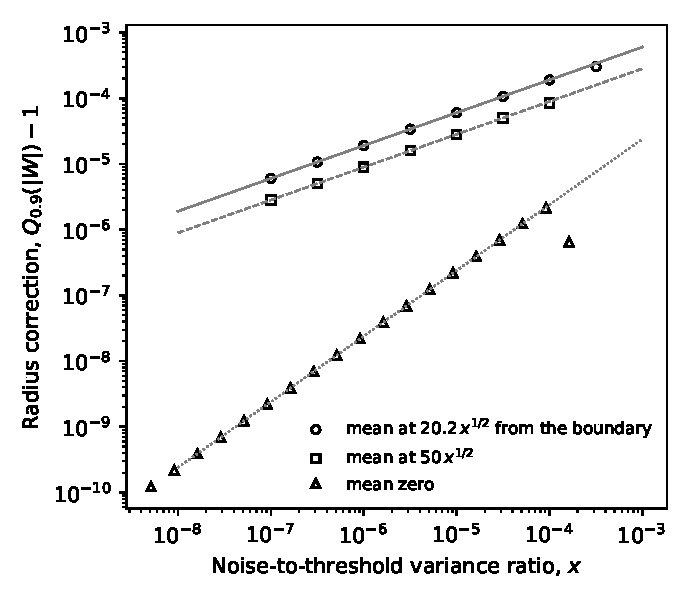
\includegraphics[width=0.6\textwidth]{fig_mean_location.pdf}
\caption{Radius correction $Q_{0.9}(|W|) - 1$ against $x$ on logarithmic axes, for laws with noisy coverage exactly $0.9$: mean at $20.2\,x^{1/2}$ from the boundary (circles), at $50\,x^{1/2}$ (squares) and mean zero (triangles), with $c_{0.9}x^{1/2}$ (solid), $L_{0.9}(50)x^{1/2}$ (dashes) and $0.024\,x$ (dots). Only positive corrections are shown.}
\label{fig:s-mean}
\end{figure}

\subsection*{The limit with $\kappa$ fixed}

The limit in Theorem~\ref{M-thm:transition} is taken with $\kappa$ fixed. Applying the small-$u$ construction to a centred law, that is, $\kappa = x^{-1/2}$, gives in the limit a left exponential tail of rate $1 - \log(1/q)$ whose noise-free central coverage is $q\{1 - e^{-2 + 2\log(1/q)}\}$, $0.750$ at $q = 0.9$, far below the constraint. So $\{1 - \log(1/q)\}/2$ is not a lower bound for the centred coefficient.

\section{Certification}\label{sec:s-cert}

\subsection*{Box bounds for the radius}

By the symmetry $W \mapsto -W$ of the kernel and of $|W|$ it suffices to treat $\beta \ge 0$. Write a member of $\mathcal F$ with $\beta \ge 0$ as $W = b - Y$, where $Y$ has density proportional to $e^{-\beta y}$ on $[0,\ell]$. The ends of the family are included: $\ell = 0$ or $\beta = \infty$ gives a point mass and $\ell = \infty$ an exponential tail. For slopes $\beta' > \beta$ the likelihood ratio $e^{-(\beta'-\beta)y}$ is decreasing, so $Y_{\beta'}$ lies below $Y_\beta$ in likelihood-ratio order, and for lengths $\ell < \ell'$ truncation gives $F_\ell \ge F_{\ell'}$. Thus $W$ is stochastically increasing in $\beta$ and $b$ and decreasing in $\ell$. On a box of parameters let $W_{\rm lo}$ and $W_{\rm hi}$ be the stochastically smallest and largest corners. Since $\pr(W + e \le \pm 1)$ and $\pr(W \le y)$ are expectations of decreasing functions of $W$, every law in the box satisfies
\[
\pr(|W+e| \le 1) \le \pr(W_{\rm lo} + e \le 1) - \pr(W_{\rm hi} + e \le -1),\qquad \pr(|W| \le s) \ge \pr(W_{\rm hi} \le s) - \pr(W_{\rm lo} \le -s).
\]
The density bound $\pr(|W+e| \le 1) \le 2\sup f_W = 2\beta/(1 - e^{-\beta\ell})$ is also available. A box whose first bound is below $p$, or whose second bound is at least $q$, contains no law that violates $R_{p,q}(x) \le s$, and a branch and bound over boxes certifies $R_{p,q}(x) \le s$. The location is confined to $[-1 + x^{1/2}\Phi^{-1}(p), b_{\max}]$: the lower end holds because $W \le b$; for the upper end take $k = 7x^{1/2}$; the density of $W$ increases towards $b$, so $\pr(|W| \le 1+k) \le r/(1+r)$ with $r = (2+2k)/(b-1-k)$, and $\pr(|e| > k) = 2\Phi(-7)$. The parameters $\beta, \ell \in [0,\infty]$ are compactified.

\begin{proposition}\label{prop:continuity}
For all $x, h \ge 0$, $R_{p,q}(x + h) \le R_{p,q}(x) + c_q h^{1/2}$.
\end{proposition}

\begin{proof}
If $W$ is feasible at noise level $x + h$, then $W + h^{1/2}Z'$, with $Z' \sim N(0,1)$ independent of $(W, Z)$, is log-concave and feasible at level $x$. So $s = Q_q(|W + h^{1/2}Z'|) \le R_{p,q}(x)$, and Theorem~\ref{M-thm:small} at scale $s$ gives $Q_q(|W|) \le s + c_q h^{1/2}$.
\end{proof}

We computed numerical upper bounds of $R_{p,0.9}$ for $p = 0.9$, $0.9036$ and $0.9068$ on $0.002 \le x \le 0.366$ with step $5\times10^{-4}$, using Proposition~\ref{prop:continuity} between grid points. Here $0.9068$ and $0.9036$ are the order-statistic levels $p_k$ of $K = 110$, $k = 105$ at $\delta = 0.05$ and $\delta = 0.04$; the latter is used in \S~\ref{sec:s-hetero}. The closed forms agree with $30$-digit quadrature to within $10^{-11}$ at random points with $10^{-4} \le x \le 0.37$, $10^{-4} \le \ell \le 20$ or $\ell = \infty$ and $10^{-3} \le \beta\ell \le 10^{3}$, which cover the ranges in which boxes are evaluated after outward rounding (test suite; the largest error found was $1.1\times10^{-12}$), and boxes are cleared with a margin of $10^{-9}$; the bounds therefore rest on double-precision evaluation of the closed forms and are not interval arithmetic. For $0.05 \le x \le 0.3$ the bound exceeds a feasible value by at most a relative $3\times10^{-4}$ for $p = 0.9$ and $10^{-3}$ for $p = 0.9068$. The branch and bound fails only just before the feasibility edges, $x \approx 0.370$ for $p = 0.9$ and $0.361$ for $p = 0.9036$; there Proposition~\ref{prop:continuity} from the last grid point gives $R_{0.9,0.9}(x) \le 0.132$. Below $x = 0.01$ the lookup also uses Theorem~\ref{M-thm:small} and its $p \ge q$ form, which are within $0.3\%$ of a feasible value there (Fig.~\ref{fig:s-certified}). At $q = 0.9$ the numerical bounds fall below $1$ from $x = 0.013$ on, with the continuity margin $c_{0.9}(5\times10^{-4})^{1/2} \approx 4.3\times10^{-4}$ keeping them below $1$ between grid points, and reach $0.973$ at $x = 0.05$. A differential-evolution search over the three-parameter family, which evaluates the constraint by Gauss--Legendre quadrature, returned $1.027$ at $x = 0.001$, above the bound $1.0006$ of Theorem~\ref{M-thm:small}: the quadrature is inaccurate for steep slopes at small $x$. That search is therefore used only for $x \ge 0.006$, and the legacy table \texttt{results/r\_table.json} built with it is not used in the paper.

\begin{figure}[t]
\centering
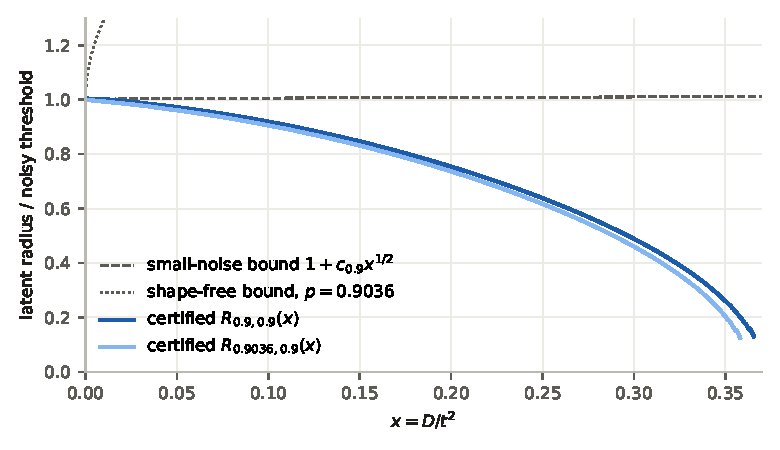
\includegraphics[width=0.7\textwidth]{fig_certified.pdf}
\caption{Numerical upper bound of the sharp radius $R_{p,0.9}(x)$ for $p = 0.9$ and for the order-statistic level $p = 0.9036$ ($\delta = 0.04$), with the small-noise bound of Theorem~\ref{M-thm:small} and the shape-free bound $1 + x^{1/2}z_{1-(p-q)/2}$, which follows from $|W| \le |V| + |e|$.}
\label{fig:s-certified}
\end{figure}

\subsection*{Ball-arithmetic certificates for the constants}\label{sec:s-ball}

Every deciding inequality is evaluated in Arb ball arithmetic; floating point only proposes points, balls are converted to doubles with outward rounding, and sums of bounds are formed as balls.
\begin{enumerate}
\item $m_u(b)$ decreases in $b$, and in $u$ because $E_u$ is stochastically decreasing in its rate. Hence $b_u(p)$ is nonincreasing in $u$, and on $[u_0, u_1]$, $b_u(p) - u^{-1}\log(1/q) \le b_{u_0}(p) - u_1^{-1}\log(1/q)$. A ball with $m_u(b) < p$ proves $b_u(p) < b$.
\item For $u \ge u_{\max}$ the value is at most $b_{u_{\max}}(p)$. For small $u$, let $b(u) = \{\log(1/p) + u^2/2 - \log(1 - u^3)\}/u$. Then $e^{-ub + u^2/2} = p(1 - u^3)$, and the Mills ratio gives $\Phi(-b) \le pu^3$ whenever $\phi\{\log(1/p)/u\} \le p\,u^2\log(1/p)$. This holds on $(0, u_{\min}]$ once it holds at $u_{\min} \le \log(1/p)/2^{1/2}$, because the left side divided by $u^2$ increases there. So $b_u(p) \le b(u)$, and for $p \ge q$ the resulting bound increases in $u$.
\item By Lemma~\ref{M-lem:onesided}, $c_{p',q'} \le \gamma$ if and only if $1 - q' \ge \varphi_\gamma(1 - p')$, where $\varphi_\gamma(a) = \max[0, \sup_u 1 - \exp\{-u(b_u(1-a) - \gamma)\}]$. Hence $C_{p,q} \le \gamma$ if $\varphi_\gamma(a_L) + \varphi_\gamma(a_R) \le 1 - q$ whenever $a_L + a_R = 1 - p$. Since $\varphi_\gamma$ is nondecreasing, it suffices to check this at the ends of an adaptive partition of $a_L$, with $\varphi_\gamma$ bounded above by the same monotone branch and bound in $u$.
\end{enumerate}
The certificates give $c_{0.8} \in [0.0460730, 0.0460731]$, $c_{0.9} \in [0.0190618, 0.0190619]$, $c_{0.95} \in [0.0084075, 0.0084077]$ and $c_{0.99} \in [0.0013950, 0.0013958]$, $-0.0571845 \le c_{0.9036,0.9} \le C_{0.9036,0.9} \le -0.057$, $-0.1149813 \le c_{0.9068,0.9} \le C_{0.9068,0.9} \le -0.114$, and $C_{q+\delta,q} \le 0$ for $(q, \delta) = (0.8, 0.005)$, $(0.9, 0.001)$ and $(0.95, 0.0002)$. Lower bounds $c_{q+\delta,q} > 0$ at $\delta = 0.0043$, $0.00079$ and $0.00015$ come from single points $u$, evaluated in ball arithmetic, and $C_{p,q} \ge c_{p,q}$. Double-precision root finding puts the smallest slack at $4.4\times10^{-3}$, $8.0\times10^{-4}$ and $1.6\times10^{-4}$.

\section{Heterogeneous and estimated noise variances}\label{sec:s-hetero}

\subsection*{Heterogeneous known variances}

In the heterogeneous rule, $\varepsilon$ bounds, for each data set, the sup-norm error of the average kernel after compressing the $D_i$ to $32$ support points: the maximum over a grid of spacing $h = 10^{-3}$ plus $Mh^2/8$, with $M$ a bound on the second derivative; it was about $2\times10^{-4}$. For each data set a numerical upper bound of $R^{\rm mix}$ is computed by the box bounds, which hold term by term for a mixture kernel, and the shape-free bound is used if the branch and bound fails.

Replacing the average kernel by the kernel of a single variance is not safe. With the mean variance plugged in, the radius is $1.4\%$ too short at mean $x = 0.2$ with lognormal spread $1$ (numerical). The smallest variance also fails: take $W = b - E_2$ with $b = 1.0435647$ and noise an equal mixture of $N(0, 10^{-8})$ and $N(0, 5\times10^{-4})$. The noisy coverage of $[-1, 1]$ exceeds $0.9$, while the radius $1 + c_{0.9}10^{-4}$ given by the smaller variance covers $W$ with probability $0.89977$; this was checked in $192$-bit ball arithmetic.

\subsection*{Estimated variances}

Suppose the $D_i$ are unknown and estimates $\hat D_i$ are available that are independent of the scores, as for the sample means and variances of normal unit data. The order-statistic event of Proposition~\ref{M-prop:beta} involves the scores only. Let $\mathcal E_\eta$ be an event determined by the $\hat D_i$ with $\pr(\mathcal E_\eta) \ge 1 - \eta$.

\begin{lemma}\label{lem:dominate}
Let $G \in \LC$. Suppose that on $\mathcal E_\eta$ a continuous kernel $u_t$, vanishing at $\pm\infty$, satisfies $u_t \ge \bar g_{D,t}$ pointwise for every $t > 0$. Then $s = T\,R_{p_k,q}[u_T]$, the radius \eqref{M-eq:R} with kernel $u_T$, covers a new latent residual with probability at least $q$, conditionally on the data, with probability at least $1 - \delta - \eta$. If $\mathcal D_\eta$ is a confidence set with $\pr(D \in \mathcal D_\eta) \ge 1 - \eta$, the same holds for $s = T\sup_{d \in \mathcal D_\eta} R^{\rm mix}_{p_k,q}(d/T^2)$. With a compressed kernel, $p_k$ is replaced by $p_k - \varepsilon$ as in \S~\ref{M-sec:hetero}.
\end{lemma}

\begin{proof}
On both events, $\int u_T\,dG \ge \int \bar g_{D,T}\,dG \ge p_k$, and Proposition~\ref{M-prop:reduction} applies to $u_T$. The union bound gives $1 - \delta - \eta$, with no independence between the two events needed.
\end{proof}

\begin{lemma}\label{lem:scale}
For $\lambda \ge 1$, $R^{\rm mix}_{p,q}(\lambda x_1, \ldots, \lambda x_K) \le \lambda^{1/2} R^{\rm mix}_{p,q}(x_1, \ldots, x_K)$.
\end{lemma}

\begin{proof}
If $W$ is feasible at $\lambda x$, then $U = \lambda^{-1/2}W$ satisfies the constraint at threshold $\lambda^{-1/2} \le 1$, hence at threshold $1$, so $Q_q(|W|) = \lambda^{1/2}Q_q(|U|) \le \lambda^{1/2}R^{\rm mix}_{p,q}(x)$.
\end{proof}

A confidence box for all $K$ variances needs level $1 - \eta/K$ per area and is useless with one or two degrees of freedom. Survey practice instead models variances through a few parameters, as generalized variance functions do. In the simplest such model $D_i = \sigma^2 a_i$ with known $a_i$, for instance $a_i = 1/n_i$, and the pooled estimate satisfies $\nu\hat\sigma^2/\sigma^2 \sim \chi^2_\nu$ with $\nu = \sum_i(n_i - 1)$. The confidence set is the segment $\{\sigma^2 a : \ell \le \sigma^2 \le h\}$. Lemma~\ref{lem:scale} covers the supremum over it by finitely many points without assuming that $R$ is monotone in $\sigma^2$: for $\ell = s_0 < \cdots < s_m = h$,
\[
\sup_{\ell \le \sigma^2 \le h} R^{\rm mix}_{p_k,q}(\sigma^2 a/T^2) \le \max_j\,(s_{j+1}/s_j)^{1/2}\,U_j, \qquad U_j \ge R^{\rm mix}_{p_k,q}(s_j a/T^2).
\]
Plugging in the lower end $\ell$ alone would not be justified, since $R$ can increase with the noise level (Theorem~\ref{M-thm:small}).

In simulations, areas have $n_i$ normal units, so $D_i = \sigma_i^2/n_i$ and the within-area variances are independent of the direct estimates; $K = 110$, mean $D = 0.577$, and $100$ replications per setting and law (normal, Laplace, truncated Laplace). The rule uses $\delta = 0.04$ and $\eta = 0.01$, split as $0.009$ below and $0.001$ above the pooled interval for $\sigma^2$, and needs $18$ grid points on average. The radii below use converged grid values at those points; for the first $30$ data sets of every setting and law ($270$ in all) the rule was rerun with numerical upper bounds $U_j$ at every grid point, as Lemma~\ref{lem:dominate} requires. The branch and bound succeeded for every data set, and the half-width grew by $0.14\%$ on average and by at most $1.0\%$, at about $3.6$ minutes per data set on one core.
\begin{enumerate}
\item With $n_i \in \{2, 3\}$, $\nu \approx 165$, the rule is $6.3$--$6.5\%$ shorter than noisy conformal calibration and $2.9$--$3.0\%$ longer than the known-variance rule at the same level, which is $9.0$--$9.1\%$ shorter than noisy conformal calibration. With $n_i \in \{5, \ldots, 10\}$, $\nu \approx 740$, the figures are $7.1$--$7.7\%$ and $1.6$--$1.7\%$. Relative to the known-variance rule at $\delta = 0.05$, which needs no budget for the variances and meets the same final target, $62$--$63\%$ and $73$--$74\%$ of its gain survive. Reliability of the rule with grid values was at least $0.98$; with numerical upper bounds, on the $30$ data sets per setting, it was at least $0.967$.
\item The supremum over the interval exceeded the value at its lower end by $0.2\%$.
\item When the within-area variances differ, with lognormal spread $0.5$, the common-variance model is wrong and no guarantee applies; the rule was still reliable, at least $0.99$, and $5.9$--$6.5\%$ shorter than noisy conformal calibration.
\item Without pooling, with each area's variance estimated from $\nu$ own degrees of freedom, a kernel envelope built from area-wise intervals and a binomial bound on the number of misses is $31$--$40\%$ longer than noisy conformal calibration at $\nu = 2$, within $1.3\%$ of it at $\nu = 50$, and $4.7$--$5.0\%$ and $6.6$--$7.2\%$ shorter at $\nu = 200$ and $1000$ ($30$ replications per law; grid values). Whether a better area-wise construction exists is open.
\end{enumerate}

\section{The shape-free comparison rule}\label{sec:s-shapefree}

\begin{proposition}\label{prop:shapefree}
Let $\bar g$ be a kernel that is symmetric, continuous, strictly decreasing in $|w|$ and tends to $0$ as $|w| \to \infty$, with $m = \bar g(0)$, and suppose that $qm < p < m$. Over all laws $G$ on the real line with $\int \bar g\,dG \ge p$, the supremum of $Q_q(|W|)$ is the radius $r$ that solves $\bar g(r) = (p - qm)/(1 - q)$.
\end{proposition}

\begin{proof}
Let $\tau = (p - qm)/(1-q) \in (0, m)$. Since $m - \bar g(W) \ge 0$, Markov's inequality gives $\pr\{\bar g(W) < \tau\} \le \{m - p\}/(m - \tau) = 1 - q$, and $\bar g(W) < \tau$ exactly when $|W| > r$, so $Q_q(|W|) \le r$. Conversely, for small $\epsilon > 0$ put mass $q - \epsilon$ at $0$ and mass $1 - q + \epsilon$ at the point $w_\epsilon > 0$ with $\bar g(w_\epsilon) = \{p - (q - \epsilon)m\}/(1 - q + \epsilon)$. This law meets the constraint with equality, has $Q_q(|W|) = w_\epsilon$, and $w_\epsilon \to r$ as $\epsilon \to 0$.
\end{proof}

The average kernel of \S~\ref{M-sec:hetero} satisfies these conditions, so for a fixed rank the shape-free rule of Table~\ref{M-tab:synth} is the smallest radius that the single order-statistic constraint allows without a shape assumption. With $1$ in place of $\bar g(0)$ it contains the bound of \citet{guille2024}. It is not a bound on procedures that use several thresholds or tune the rank on independent data, as LatentCP \citep{zheng2026} can.

\section{Simulation details and an application}\label{sec:s-sim}

\subsection*{Table 1}

Conditional coverage is computed from closed-form latent distribution functions. With $150$ data sets the binomial standard error of a reliability is $0.018$ at $0.95$ and at most $0.029$ at the lowest reliability observed, $0.847$; for instance $145/150 = 0.967$ has the $95\%$ binomial interval $[0.924, 0.989]$. The computed radius uses the order-statistic level $p_k = 0.9068$ of $\delta = 0.05$. The branch and bound returned a numerical upper bound of $R^{\rm mix}$ for every one of the $1050$ data sets, at relative tolerance $10^{-3}$ in $671$, $3\times10^{-3}$ in $363$ and $10^{-2}$ in $16$, so the shape-free fallback was never used. With the mean variance in a single Gaussian kernel, which is not a valid plug-in, the numerical radius at level $p_k$ is $2.9$--$3.0\%$ shorter than at level $p = q$ (\texttt{LDC\_cert\_pk} against \texttt{LDC\_PAC} in \texttt{results/hetldc\_synth\_summary.csv}), so most of the gain over a $p = q$ calibration comes from the order-statistic level. The shape-free rule was run at every fixed rank $106$--$110$ and all results are stored; rank $107$ is reported because it is best on average over the first four laws, which favours the comparison rule. The Fay--Herriot interval falls short of the target under the Laplace law by about $1.3$ standard errors and under the truncated Laplace law, with reliability $0.847$, by about $5.8$. The Fay--Herriot tolerance interval is our adaptation of the parametric bootstrap of \citet{chatterjee2008} to an intercept-only model: the bootstrap $(1-\delta)$-quantile of the multiplier each refit needs to cover $N(\hat\mu, \hat A)$ with probability $0.9$. The latent residuals are drawn directly, with no fitted centre, and the mean noise variance $0.577$ matches the ratio of design to model variance in the application below.

\subsection*{Reliability of the analytic rules with $2000$ data sets}

The noisy threshold, Corollary~\ref{M-cor:simple} and the Markov rule need no numerical optimization, so \texttt{experiments/e36\_analytic\_reliability.py} reran them on $2000$ fresh data sets for each of the seven laws of Table~\ref{M-tab:synth}. Every rule reached conditional coverage $0.9$ in all $2000$ data sets for every law, so each reliability has Clopper--Pearson $95\%$ interval $[0.998, 1]$, including the $t_3$ law, outside $\mathcal B$. Mean conditional coverage was $0.969$--$0.992$ for the noisy threshold, $0.968$--$0.991$ for Corollary~\ref{M-cor:simple} and $0.984$--$0.999$ for the Markov rule, and the $5\%$ quantile of conditional coverage was at least $0.947$, $0.945$ and $0.968$. The guarantees are therefore conservative in these designs: the latent laws are far from the extremal laws of \S~\ref{M-sec:mean}.

\subsection*{Oracle-matched widths}

In a larger experiment with seven latent shapes, common and heterogeneous noise and $2000$ data sets per setting, each rule's width was rescaled by a single factor, chosen with knowledge of the latent law, to reach reliability $0.95$ exactly. At matched reliability, marginal noisy conformal calibration was shortest in $12$ of the $14$ settings and the Fay--Herriot tolerance interval in the other $2$; relative to noisy conformal calibration the Fay--Herriot tolerance interval was $3.1\%$ shorter to $12.1\%$ longer and the log-concave rule $4.5$--$11.5\%$ longer (\texttt{results/conditional\_synth\_exact\_matched.csv}). The log-concave rule with its guarantee was a median $15\%$ (range $9$--$33\%$) wider than its own oracle-matched width, and the Fay--Herriot tolerance interval a median $6\%$ (range $-3$ to $16\%$). So the advantage of the log-concave rule over noisy conformal calibration lies in obtaining a latent guarantee cheaply, not in a better interval shape.

\subsection*{Comparison with LatentCP and deconvolution}

\texttt{experiments/e34\_competitors.py} runs the following rules on the $600$ data sets of the first four laws of Table~\ref{M-tab:synth}; widths are relative to the computed radius. For the other three laws only the two analytic rules were run.
\begin{enumerate}
\item LatentCP \citep{zheng2026}, single level with $\gamma = \alpha/2$, has a marginal guarantee. Its latent set depends on the new unit's noise variance, which an unsampled area does not have; we draw it from the distribution that generated the $D_i$, $400$ draws per data set, and average coverage and width over the draws. It was $16$--$18\%$ longer, with mean coverage $0.976$--$0.990$ and reliability $1.0$. The tuned single-level and two-level versions, tuned on half the data, were $15$--$25\%$ longer. A PAC version with a binomial rank, our adaptation, was $39$--$58\%$ longer.
\item The deconvolution threshold of \citet{cohen2025}, with the mixture kernel in place of their homoscedastic kernel, collapses at $K = 110$ with their bin width $0.01$: most bins are empty and the masked fit gives mean coverage $0.32$--$0.44$. With bin width $0.2$ and the empty bins fitted as zeros it had mean coverage $0.88$--$0.90$, reliability $0.45$--$0.67$ and width $22$--$30\%$ shorter; it has no latent guarantee.
\item The noisy threshold of Proposition~\ref{M-prop:unknown} was $10.5$--$11.7\%$ longer and Corollary~\ref{M-cor:simple} $9.1$--$10.2\%$ longer, both with reliability $1.0$.
\end{enumerate}
The tuning grids of LatentCP and the scan step $0.01$ of the deconvolution threshold are our choices; the original papers do not fix them for this setting.

\subsection*{School districts}

In the finite population \texttt{apipop} \citep{lumley2004}, $110$ of $325$ school districts are used for training and $110$ for calibration, with $2$ or $3$ schools sampled per district. Coverage is the share of the remaining $105$ districts that are covered. Design variances are estimated with $1$--$2$ degrees of freedom and plugged in as known by every rule, a case that no guarantee covers. Over four conditions of $120$ replications, the reliability of the heterogeneous rule was $0.942$--$0.992$, of the mean-variance rule $0.983$--$1.000$ and of the Fay--Herriot interval $0.908$--$0.992$, below target in two conditions. The heterogeneous rule at level $p_k$ was $0.8$--$5.2\%$ shorter than the mean-variance rule with the $p = q$ table, mostly because of the level, and $10$--$16\%$ longer than the Fay--Herriot interval.

\section{Reproducibility}\label{sec:s-code}

All computations are in the public repository \texttt{https://github.com/kunhailP/noisy-calibration-latent-coverage}. The core routines are in \texttt{src/uai}: closed forms and the transition coefficient in \texttt{extremal.py}, the box certificates in \texttt{certify.py}, ball arithmetic in \texttt{interval.py}, and the procedures in \texttt{procedures.py} and \texttt{estimated.py}. The test suite, run by \texttt{make test}, checks the constants, the counterexamples and the centring bounds, and the \texttt{Makefile} lists the command that produces each group of results. The experiments are numbered scripts in \texttt{experiments}; \texttt{e27} produces the ball-arithmetic certificates, \texttt{e24} and \texttt{e25} the certified tables, \texttt{e20} Table~\ref{M-tab:synth}, \texttt{e29} and \texttt{e30} the estimated-variance results, \texttt{e31} the shape-free rule, \texttt{e32} the centring and transition values, \texttt{e34} the comparison with LatentCP and deconvolution, \texttt{e35} and \texttt{fig\_mean\_location.py} Fig.~\ref{fig:s-mean}, and \texttt{fig\_transition.py} Fig.~\ref{M-fig:transition}. The analytic rules of Proposition~\ref{M-prop:unknown} and Corollary~\ref{M-cor:simple} are \texttt{noisy\_threshold\_halfwidth} and \texttt{simple\_shrink\_halfwidth} in \texttt{procedures.py}; \texttt{hetldc\_certified} gives the computed radius, while \texttt{hetldc\_halfwidth} returns a grid value, a lower bound of $R^{\rm mix}$, and is not a guaranteed radius.

\bibliographystyle{biometrika}
\bibliography{refs}

\end{document}
